
\chapter{Accelerator Physics Fundamentals}\label{ch:accelerator_physics_fundamentals}

\section{Particle motion and Frenet-Serret co-ordinate system}

The standard choice of co-ordinates in accelerator physics, which takes advantage on the toroidal symmetry of the circular accelerator system, is the Frenet-Serret co-ordinate system.

Starting from the Cartesian system $(X,\, Y,\, Z)$, centred in the accelerator centre, the Frenet-Serret co-ordinate system considers as one curvilinear co-ordinate the reference orbit $s$, which describes the ideal longitudinal motion of a particle inside the accelerator, and two Cartesian co-ordinates $x$ and $y$ for the transverse one. In Fig.~\ref{fig:frenserr}, we illustrate the co-ordinate system applied to a vector $\vb{r}$.

Mapping the Cartesian system to the Frenet-Serret co-ordinate system reads:
%
\begin{equation} 
    X = (x+\rho)\cos(\frac{s}{\rho})\,, \qquad Y=y\,, \qquad Z=(x+\rho)\sin(\frac{s}{\rho})\,.
\end{equation}

To keep the particles on a reference orbit of radius $\rho$, a linear electromagnetic field of intensity $B$ is applied. $\rho$ then is given by the equilibrium between the magnetic and the centrifugal force. This equilibrium is expressed within the quantity $B\rho$, defined as \textit{beam rigidity}, which corresponds to
\begin{equation}
    B\rho = \frac{p}{e}
    \label{eq:beam_rigidity}
\end{equation}
where $p$ is the particle momentum and $e$ its charge.

Starting from this co-ordinate system, it is possible to achieve a practical Hamiltonian expression for a particle in an accelerator.

\begin{figure}
\centering
\def\svgwidth{0.75\columnwidth}
\import{2_accelerator_physics_fundamentals/figs/}{fernet_nuovo.pdf_tex}
\caption{The Frenet-Serret co-ordinate system applied to a vector $\vb{r}$ in the starting Cartesian system. The reference orbit represents an ideal particle trajectory in the accelerator, whose curvature radius is $\rho$. The $s$ co-ordinate is measured along the trajectory while $x$ and $y$ are orthogonal to it.}
\label{fig:frenserr}
\end{figure}

Let us begin from the Hamiltonian of a relativistic charged particle under the effect of an electromagnetic field, which acts via the Lorentz force. The particles are accelerated in modulus by the action of an electric field $\mathbf{E}$ (or by the scalar potential $\Phi$), and their trajectories are bent, in order to keep them on the reference circular orbit, by a magnetic field $\mathbf{B}$, which can be expressed via the vector potential $\mathbf{A}$, i.e.\ $\mathbf{B}=\rot\mathbf{A}$.

The Hamiltonian for a relativistic particle under Lorentz force reads
%
\begin{equation}
    \ham = e\Phi + \sqrt{ m^2c^4 + (c\mathbf{p}-e\mathbf{A})^2 }\,. 
\end{equation}
%
We then express the square norm of $(c\mathbf{p}-e\mathbf{A})$ in the Frenet-Serret system of co-ordinates $(x,\,y,\,s)$, whose metric tensor reads
%
\begin{equation} 
    g_{ij} = \mathrm{diag}\qty(1,\,1,\,1+\frac{x}{\rho})\,. 
\end{equation}
%
Leading to,
%
\begin{equation}
    \ham = e\Phi + \sqrt{ m^2c^4 + \frac{(cp_s-eA_s)^2}{(1+x/\rho)^2 } + (cp_x-eA_x)^2+ (cp_y-eA_y)^2}\,.
    \label{eq:ham_process_1}
\end{equation}
%
It is convenient from this point forward to treat $s$ as the time co-ordinate. Consequently, due to canonical coupling, the conjugated momentum $-p_s$ will work as the Hamiltonian function $\tilde\ham$. Solving Eq.~\eqref{eq:ham_process_1} for $p_s$, we obtain
%
\begin{equation} 
    \tilde{\ham} = -\qty(1-\frac{x}{\rho})\sqrt{\frac{E^2}{c^2}-m^2c^2-(p_x-eA_x)^2-(p_y-eA_y)^2} - eA_s\,,
\end{equation}
%
where $E=\ham-e\Phi$. We have from special relativity that $E^2/c^2 = p^2 + m^2c^2$,this allows us to rewrite the Hamiltonian as
\begin{equation}
    \tilde{\ham} = -\qty(1-\frac{x}{\rho})\sqrt{p^2-(p_x-eA_x)^2-(p_y-eA_y)^2} - eA_s\,.
\end{equation}

In high-energy circular accelerators, like the ones considered for this study, the motion in the longitudinal direction is far faster than in the transverse ones, i.e.\ $p\gg p_x$ and $p\gg p_y$. This enables the $\sqrt{1+x}\approx 1+x/2$ expansion for Hamiltonian, leading to
%
\begin{equation} 
	\tilde\ham = \qty(1+\frac{x}{\rho})\qty[-p + \frac{1}{2p}\qty(p_x^2+p_y^2)] -eA_s\,. 
	\label{eq:hamem}
\end{equation}

If we are considering only transverse effects, we can assume that there is no magnetic field in the longitudinal direction. With this assumption, we only have contributions to the vector potential along $s$, and $A_x=A_y=0$, i.e.\ $\mathbf{B}=(B_x,\,B_y,\,0)$.

A practical approach for evaluating the magnetic field contribution to $\tilde\ham$, $eA_s$, consists in expanding the magnetic field in its multipolar components.

From Maxwell's equation $\rot\mathbf{B}=0$, one gets the Laplace equation $\laplacian\mathbf{A}$, which, for $A_s$ has the general solution that can be expressed in power series as
%
\begin{equation}
	A_s = \Re\sum_{n}\qty[ \frac{k_n + ij_n}{(n+1)}(x+iy)^{n+1}]\, ,%%%TODO::controlla def
	\label{eq:as}
\end{equation}
%
which leads to the corresponding expansion of the magnetic field
\begin{equation}
	B_y + iB_x = \sum_n (k_n + ij_n) (x+iy)^n\,.
\end{equation}
%
The coefficients
\begin{equation}
	k_n = \frac{1}{n!} \pdv[n]{B_y}{x}\eval_{x=y=0}, \qquad 
	j_n = \frac{1}{n!} \pdv[n]{B_x}{y}\eval_{x=y=0} 
\end{equation}
%
are called, respectively, the \textit{normal} and \textit{skew} $2(n+1)$-polar coefficients of the magnetic field. In accelerator physics literature, usually considers magnetic elements that generate fields with only one multipolar component. These elements are in fact referred to as normal or skew dipoles, quadrupoles, sextupoles, octupoles and so on.

%
\section{Transverse motion definition}
%

From the Hamiltonian \eqref{eq:hamem}, we can derive the equations of motion of the particle in the transverse plane. We obtain
%
\begin{equation}
    \begin{aligned}
        x' &= \qty(1+\frac{x}{\rho})\frac{p_x}{p}\,, &\qquad p_x' &= \frac{p}{\rho}\qty(1+\frac{x}{\rho}) + e\pdv{A_s}{x}\,,\\ % TODO::CHECK
        y' &= \qty(1+\frac{x}{\rho})\frac{p_y}{p}\,, &\qquad p_y' &= e\pdv{A_s}{y}\,.
    \end{aligned}
    \label{eq:ham_motion}
\end{equation}

In order to get an expression for the partial derivatives of $A_s$ as a function of the $x$ and $y$ components of the magnetic field $\mathbf{B}$, we consider the expression of $\curl \mathbf{A}$ in Frenet-Serret co-ordinates, which reads
%
\begin{equation}
    \curl \mathbf{A} = \frac{\hat x}{1+x/\rho}\pdv{A_s}{y} - \frac{\hat y}{1+x/\rho}\pdv{A_s}{x} = B_x\hat x + B_y\hat y % TODO::CHECK
\end{equation}
%
as only the $A_s$ component is non-zero. This leads to
%
\begin{equation}
    \pdv{A_s}{x} = -\qty(1+\frac{x}{\rho})B_y\,, \qquad \pdv{A_s}{y} = \qty(1+\frac{x}{\rho})B_x\,,
\end{equation}
%
which, substituted in Eq.~\eqref{eq:ham_motion}, reads
%
\begin{equation} 
    \begin{aligned}
        x' &= \qty(1+\frac{x}{\rho})\frac{p_x}{p}\,, &\qquad p'_x &= \qty(1+\frac{x}{\rho})\qty[ \frac{p}{\rho} - eB_y]\\
        y' &= \qty(1+\frac{x}{\rho})\frac{p_y}{p}\,, &\qquad p'_y &= e\qty(1+\frac{x}{\rho})B_x\,.
    \end{aligned}
\end{equation}
%
Recalling the definition of the beam rigidity in Eq.~\eqref{eq:beam_rigidity}, we can rewrite the equations as second order differential equations using the fact that $p=eB\rho$. This leads to
%
\begin{equation}
    \begin{split}
        x'' &= \frac{1}{\rho} + \frac{x}{\rho^2} + \frac{B_y}{B\rho}\qty(1+\frac{x}{\rho})^2\,,\\
        y'' &= \frac{B_x}{B\rho}\qty(1+\frac{x}{\rho})^2\,.
    \end{split}
    \label{eq:acc_step_1}
\end{equation} 

If we consider only linear terms for the magnetic fields $B_x$ and $B_y$, these equations can be expressed in the form 
\begin{equation}
	z''+K_z(s)z = 0\, ,
    \label{eq:acc_step_2}
\end{equation}
where $z$ stands for either $x$ or $y$, and the function $K(s)$ represents the effect of the linear magnetic fields the particle is subject to in the accelerator.  For a circular accelerator of length $L$ the periodic condition $K_z(s)=K_z(s+L)$ holds. This equation with the periodic condition is referred in literature as \textit{Hill's equation}.


An Ansatz for the solution of Hill's equation is in the form
\begin{equation}
	z(s)=A\sqrt{\beta_z(s)}\cos\left(\psi_z(s)\right)\,,
	\label{eq:hill_zeta}
\end{equation}
%
\ie a harmonic oscillator where the amplitude $\beta_x(s)$ and phase advance $\psi_z(s)$ is dependent on $s$. Which, substituted into Hill's equation results in a relation between $\psi_z(s)$ and $\beta_z(s)$,
%
\begin{equation}
	\frac{1}{\sqrt{\beta_z(s)}} \dv{s}(\beta_z(s)\psi_z(s)) = 0\,,
\end{equation}
%
which can be solved as
%
\begin{equation}
	\psi_z = \int_0^s \frac{\dd s'}{\beta_z(s')}\,
\end{equation}
%
and a non-linear equation for $\beta_z(s)$:
%
\begin{equation}
	\frac{1}{2}\beta_z\beta_z''-\frac{1}{4}\beta_z'^2+K_z(s)\beta_z^2=1\,.
\end{equation}

The phase advance over the ring is called \textit{tune}:
\begin{equation}
	\nu_z = \frac{1}{2\pi}\oint \frac{\dd s'}{\beta_z(s')}\,.
    \label{eq:tune_def}
\end{equation} 


\section{Courant-Snyder ellipse}

Solving $\beta_z(s)$ only determines the scaling of the solution $z(s)$ given in \eqref{eq:hill_zeta} at each value $s$. As we are interested in the particle transverse motion, we want to consider its evolution each time it crosses the position $s=s_0$, i.e.\ we want to consider the Poincaré section of the dynamics. At each iteration, we will have a phase advance of $\psi_z$ equal to $2\pi\nu_z$.

It is possible to decouple the envelope dynamics described by $\beta_z(s)$ from the particle transverse motion with a co-ordinate transformation, which leads to the definition of the Courant-Snyder ellipse, and other important objects in accelerator physics.

Starting from Eq.~\eqref{eq:hill_zeta}, we have that the momentum $z'(s)$ reads
%
\begin{equation}
	z'(s)=-\frac{z}{\beta_z(s)}\qty(\alpha_z(s)+\tan\psi_z(s))\,
\end{equation}
%
where $\alpha_z=-\beta'_z/2$. We then consider for our co-ordinate transformation the angular variable $\phi_z=\psi_z$ and the generating function
%
\begin{equation}
	F=\int \dd z\, z' = -\frac{z^2}{2\beta_z}(\alpha_z+\tan\phi_z) \,,
\end{equation}
%
which then yields the canonical action variable $I_z$, which then reads
%
\begin{equation}
	I_z=\pdv{F}{\phi_z}=\frac{z^2}{2\beta_z}(1+\tan^2\phi_z)=\frac{1}{2\beta_z}\qty[z^2+(\beta_z z'+\alpha_z z)^2]\,.
	\label{eq:jz}
\end{equation}

In the new variables, the Hamiltonian of Hill's equation
\begin{equation} 
    \ham = \frac{z'^2}{2} + \frac{K_z z^2}{2} \,,
\end{equation}
taking into account the derivative $\pdv*{F}{s}$, reduces to the simple expression
\begin{equation}
	\ham(\phi,I,s) = \frac{I}{\beta(s)}\, .
\end{equation}
From this new Hamiltonian, we have that the equation of motion for the variable $\phi_z$ reads $\phi'_z = 1/\beta(s)$. We are now interested in making $\phi_z$ proportional to $s$, and remove any dependence from the $\beta$ function in the equations of motion.

To achieve this, we define the frequency
\begin{equation}
    \omega_z = \frac{2\pi\nu_z}{L} \,,
\end{equation}
where, we recall, $L$ is the circumference of the accelerator and $\nu_z$ the tune defined in Eq.~\eqref{eq:tune_def}. We then have the final change of variables $(\phi_z,I_z)\to(\tilde\phi_z, \tilde I_z)$, which is given by the generating function
%
\begin{equation}
	G(\phi_z,\tilde I_z) = \tilde I_z\qty(\omega_z s - \int_0^s\frac{\dd s'}{\beta(s')})+\phi\tilde I\, ,
\end{equation}
%
which results in the Hamiltonian
%
\begin{equation}
	\ham(\tilde \phi_z,\tilde I_z) = \omega_z \tilde I_z\,,
	\label{eq:harm_ham}
 \end{equation}
%
which is the well known Hamiltonian of a harmonic oscillator (note how $I_z$ = $\tilde{I}_z$).

From this final Hamiltonian, one can introduce and operate with normalized Cartesian co-ordinates 
\begin{equation}
    \hat z=\sqrt{2I_z}\cos\tilde{\phi}_z\,,\quad \hat p_z=\sqrt{2I_z}\sin\tilde{\phi}_z \,,
    \label{eq:2:cart_eq}
\end{equation}
and treat consequently the transverse linear motion on both the $x-p_x$ and $y-p_y$ planes using an intuitive normalized Cartesian Hamiltonian
%
\begin{equation}
	\ham(\hat x,\, \hat p_x,\, \hat y,\, \hat p_y) = \frac{\omega_x}{2}(\hat x^2 +\hat p_x^2) + \frac{\omega_y}{2}(\hat y^2+\hat p_y^2)\, .
	\label{eq:linham}
\end{equation}
%

\begin{figure}
    \centering
    \def\svgwidth{0.75\columnwidth}
    \import{2_accelerator_physics_fundamentals/figs/}{ellisse.pdf_tex}
    \caption{The Courant-Snyder ellipse $\gamma z^2 + 2\alpha zz' + \beta z'^2=2I_z$. The area enclosed by the ellipse is equal to $2\pi I_z$. }
    \label{fig:coursnyd}
\end{figure}


The Hamiltonian of Eq.~\eqref{eq:linham} describes circular trajectories in the decoupled phase spaces $(\hat x,\,\hat p_x)$ and $(\hat y\,, \hat p_y)$. Moreover, two corresponding action variables, namely,
\begin{equation}
    I_x = \frac{\hat x^2 +\hat p_x^2}{2}\,, \quad I_y=\frac{\hat y^2+\hat p_y^2}{2} \,,
\end{equation}
can be defined. $I_x$ and $I_y$ follow the standard definition of the trajectory area divided by $2\pi$ are conserved. For historical reasons, however, the value $2I_z$ is called the \text{Courant-Snyder invariant}.

Following its definition in the physical co-ordinates $(z,\, z')$, given in Eq.~\eqref{eq:jz}, it is possible to draw the constant-$I$ surfaces in the $(z,z')$ phase space, as in Fig.~\ref{fig:coursnyd}, which correspond to concentric ellipses, as its expanded form reads:
%
\begin{equation}
I_z = \frac{1}{2\beta_z}\qty[z^2 + (\alpha z + \beta z'))^2] = \frac{1}{2}\qty(\gamma z^2 + 2\alpha z z' + \beta z'^2)\,, \end{equation}
%
where we have defined $\gamma=(1+\alpha^2)/\beta$. The area of the ellipse is equal to $2\pi I_z$, and is conserved at any value of $s$. It can be observed, finally, how the $(z,z')\to(\hat z,\hat p_z)$ co-ordinate transformation modifies the physical co-ordinates ellipses into circles with the same area, from which their name \textit{``normalized co-ordinates''}.

A single particle following the linear transversal dynamics will have its own constant Courant-Snyder invariant. When instead we want to consider a beam distribution, a standard property, called \textit{emittance} is defined as the average of the Courant-Snyder invariant:
\begin{equation}
    \eps_z = \av{I_z} \,.
\end{equation}
The emittance is related to the second moments of the beam distribution in $(\hat z,\hat p_z)$. In fact, averaging over $I_z$ and $\phi_z$ in the definitions of $\hat z$ and $\hat p_z$ given in Eq.~\eqref{eq:2:cart_eq}, we obtain
%
\begin{equation}
	\av{\hat z^2} = \beta_z \eps_z, \qquad \av{\hat p_z^2}=\gamma_z \eps_z, \qquad \av{\hat z\,\hat p_z}=-\alpha_z\eps_z\,,
\end{equation}
%
from there, using the definition of $I_z$ yields
\begin{equation}
	\eps_z = \sqrt{ \av{\hat z^2}\av{\hat p_z^2} - \av{\hat z \, \hat p_z}^2 }\,.
\end{equation}

The beam emittance can then be considered either as the average Courant-Snyder invariant of a distribution, or as the area (up to a $2\pi$ factor) of the orbit of the RMS particle of the beam. A useful implication of this is that a Gaussian beam distribution in $(\phi_z,\,I_z)$ co-ordinate assumes the practical form:
%
\begin{equation}
\rho_z = \frac{1}{\eps_z}\exp(-\frac{I_z}{\eps_z})\,.
\end{equation}
%



\section{Non-linear beam dynamics}\label{sec:non-linear}

The transverse dynamics we treated so far with Hill's equation and formalism takes into consideration only the effects of a linear magnetic field (we recall the passage between Eq.~\eqref{eq:acc_step_1} and Eq.~\eqref{eq:acc_step_2}, where we dropped all the non-linear terms for the magnetic fields $B_x$ and $B_y$). This method, however, takes into account only the elements generated by a set of ideal dipole and quadrupole magnets.

To include higher order terms of the magnetic field power series, it is possible to include non-linear terms directly into Hill's Hamiltonian. This can be done in order to both represents the unavoidable higher-order magnet imperfections inside the accelerator machine, or to represent explicit sextupolar and octupolar elements one might want to include to cancel out specific sources of non-linear effects. 

As Hill's Hamiltonian is equivalent to two detached harmonic oscillators, non-linear components can be included in the Hamiltonian as anharmonic perturbation to such harmonic oscillators. We start by considering higher order terms $n \ge 2$ of the power series $A_s$, which we presented in Eq.~\eqref{eq:as}, and we perform the change of variables $(x,\,y) \to (\hat x, \hat y)$. We have then that the non-linear part of the Hamiltonian reads:
%
\begin{equation}
    \ham_\text{nlin}(\hat x, \hat p_x, s) = \Re \sum_{n\ge 2} \qty[\frac{k_n(s) + ij_n(s)}{(n+1)} \left(\sqrt{\beta_x(s)}\ \hat x + i\sqrt{\beta_y(s)}\ \hat y\right)^n]\,.
\end{equation}  

To simplify this notation, we introduce the quantity $\beta(s)=\beta_y(s)/\beta_x(s)$, and its value $\bar\beta$ averaged over an accelerator turn which reads
\begin{equation}
    \bar\beta = \oint \dd s\, \frac{\beta_y(s)}{\beta_x(s)} \,.
\end{equation}
We can now substitute the strengths $k_n(s)$ and $j_n(s)$ (which, we recall, they represent the effect of a normal or a skew $(2n+2)$-polar magnetic field) with the integrated coefficients $K_n$, $J_n$, which will be scaled by the value of $\beta_x(s)$ and $\beta_y(s)$, i.e.\ we weight the integral average with the envelope value of the beam where the magnetic elements are placed. These coefficients read
%
\begin{equation} 
	K_n = \oint \dd s\, k_n(s) \beta_x^{\frac{n+1}{2}}(s)\,,\qquad
	J_n = \oint \dd s\, j_n(s) \beta_x^{\frac{n+1}{2}}(s)\,,
\end{equation} 
%
where the integrations are evaluated over the accelerator turn. With this notation, the non-linear Hamiltonian has the simpler form
% 
\begin{equation} \ham_\text{nlin}(\hat x, \hat p_x) = \Re \sum_{n\ge 2} \qty[\frac{K_n + iJ_n}{(n+1)} (\hat x + i\bar\beta^{1/2} \hat y)^n]\,.\end{equation}

From this Hamiltonian, one can for example write a 1\textsc{d} beam model with normal multipoles
\begin{equation}
	\ham(\hat x,\hat p) = \omega \frac{\hat x^2 + \hat p^2}{2} + \sum_{n>2} K_n \frac{x^{n+1}}{(n+1)}\, ,
	\label{eq:hamxp_nl}
\end{equation}
such simple model can be used to understand many phenomenons caused by non-linear effects.

In an accelerator, non-linear effects can be used to represent either unwanted elements, such as linear magnets imperfections, or to represent specifically added non-linear magnetic elements, such as sextupoles and octupoles. Such components can be introduced inside an accelerator optics in order to correct specific unwanted effects, like \textit{chromaticity}, i.e.\ the fact that particles with different momentum are differently focused by quadrupoles. Chromaticity, specifically, can be tackled by the introduction of sextupole magnets. Another important source of non-linearities is space charge effects and \textit{beam-beam interaction} effects, caused by the electromagnetic interaction of charged particles with other charged particles, respectively in the same or in another beam during collisions.

The introduction of non-linear elements in a circular accelerator is the cause of three main effects~\cite{herr}: amplitude-dependent detuning, excitation of non-linear resonances, and reduction of the dynamic aperture. We will present the first two phenomena very briefly, and focus a little more on the core characteristics of the last one.

\subsubsection{Amplitude-dependent detuning}

Adding non-linear elements in the transverse motion has the inevitable consequence of modifying the tune, i.e.\ the rotation frequency of the harmonic oscillator, into an amplitude dependent function, where the amplitude.
The second effect of non-linear elements on transverse motion is the fact that the rotation frequency, the tune, becomes a function of the amplitude, that is, the value of the action $I$. In the linear Hamiltonian~\eqref{eq:linham}, the frequency $\Omega$ is given by
\begin{equation}
	\Omega = \pdv{\ham}{I} = \omega\,,
\end{equation}
where, we recall, $I=(\hat x^2 + \hat p^2)/2$. The tune $\omega$ is constant at any $I$, therefore particles have the same tune.

If we now add an octupolar component to the Hamiltonian, that is, an $n=3$ element of the power series in Eq.~\ref{eq:hamxp_nl}, we end up with the new Hamiltonian
\begin{equation}
	\ham = \omega \frac{\hat x^2 + \hat p^2}{2} + \frac{K_3}{5} x^4 = \omega I + \frac{K_3}{5} I^2 \cos^4\phi\, .
\end{equation}

Averaging over the angular variable $\phi$, one gets
\begin{equation}
	\av{\ham} = \omega I + \frac{3}{40}K_3 I^2,
\end{equation}
%
and
%
\begin{equation}
	\Omega(I) = \pdv{\av{\ham}}{I} = \omega + \frac{3K_3}{20} I\,.
\end{equation}
Meaning, there is now a linear dependence of the tune on the action $I$. This implies that each particle will have a different rotation frequency depending on its current amplitude.

The averaging approach used here to achieve an expression of the detuning highlights only the first-order effects in the frequency. For more complex Hamiltonians with multiple non-linear components, achieving a complete analytical expression of the detuning is not a trivial problem.

It is possible to numerically evaluate the amplitude-dependent detuning in single-particle tracking simulations, as the tune can be measured by performing a numerical estimate of the fundamental frequency of the orbit history of the transverse orbit. We will present the topic of tune evaluation later in Chapter~\ref{}, in the context of dynamic indicators, as such methods are the foundation for consolidated tools in accelerator physics like the Frequency Map Analysis.

\subsubsection{Non-linear resonances}

In an accelerator machine, it is usual to have the non-linear components at $10^{-3} - 10^{-4}$ the intensity of the linear components. However, if the tunes $\omega_x$ and $\omega_y$ are in a resonance condition, the non-linear magnetic field can lead to a geometric aberration of the phase-space and, ultimately, cause severe particle loss. A theoretical approach of this phenomenon is presented in~\cite{wilson}.

When the frequency $\omega_x$ or $\omega_y$ is close to a resonant frequency, in accordance with the Poincaré-Birkhoff theorem, chain of islands with extra fixed points appear. These islands, in regular accelerator operations, reduce the dynamic aperture (for which the definition is given in Subsection~\ref{sec:2:dynamic_aperture}) and, close to separatrices, cause the onset of chaotic motion. When a resonance is crossed due to small, undesired variations of the magnetic field, which cause oscillations in the $\omega_x$ and $\omega_y$ values, a beam amplitude growth is observed~\cite{Guignard:185921}, impacting beam lifetime.

Other than 1\textsc{d} resonances $n\omega_z \approx \ell$, where $\ell$ is an integer value, in a system with two degrees of freedom one can have a 2\textsc{d} resonant condition between the $\omega_x$ and $\omega_y$ frequencies, i.e.\ $m\omega_x-n\omega_y\approx \ell$. Only difference resonances ($m>0$, $n>0$) are stable, although they couple the motion between the two planes, while sum resonances (when $m$ and $n$ have different signs) result in unstable motion.

\begin{figure}
	\centering
	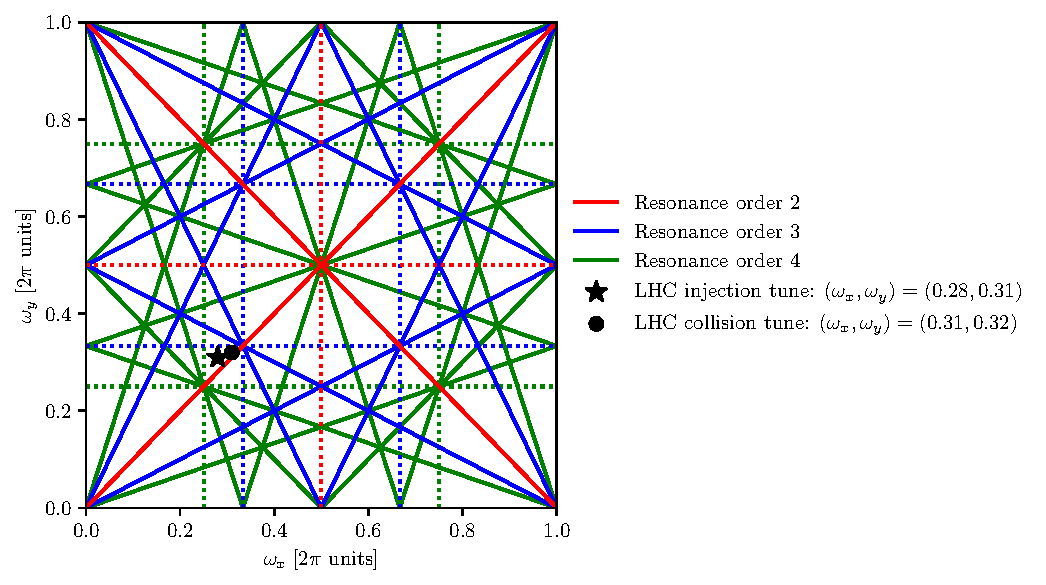
\includegraphics[width=.85\textwidth]{2_accelerator_physics_fundamentals/figs/tune_space.pdf}
	\caption{Resonance diagram in the $(\omega_x,\,\omega_y)$ space up to order $4$. The resonances are evaluated on the fractional part of $\omega_x$ and $\omega_y$. Dotted lines represent 1\textsc{d} resonances, continuous lines represent 2\textsc{d} resonances. The two characteristic working tunes for the LHC are also reported on the resonance diagram.}
	\label{fig:res}
\end{figure}

The possible 1\textsc{d} and 2\textsc{d} resonances (up to order $4$) are represented by lines in the $(\omega_x, \omega_y)$ diagram of Fig.~\ref{fig:res}, where different colours show the resonance order. As higher-order resonances are generally weaker than lower-order ones, one should select the accelerator working point quite far from the main resonances, the LHC does so by operating at the fractional tunes $(\omega_x, \omega_y)=(0.28, 0.31)$ during injection and $(\omega_x, \omega_y)=(0.31, 0.32)$ during collisions~\cite{Benedikt:823808}.

\section{One-turn maps}

A standard tool in accelerator physics to inspect the transversal dynamic of a particle in an accelerator magnetic lattice are one-turn maps. A one-turn map \(\mathrm{M}\) is the Poincaré map of the circular accelerator at section \(s = s_0\), and it is given by composing single-element maps:
\begin{equation}
	\mathrm{M} = \mathrm{M}^{(L)} \circ \mathrm{M}^{(L - 1)} \circ \cdots \circ \mathrm{M}^{(2)} \circ \mathrm{M}^{(1)} \,,
\end{equation}
which each $\mathrm{M}^{(i)}$ represents an element along the circular accelerator lattice, which might be, for example, a drift space with no magnets, a dipole bending magnet, a quadrupole, or a higher order magnetic element. 

The map \(\mathrm{M}\) transforms the phase space co-ordinates \(\vb{\hat x} = (\hat x, \hat p_x, \hat y, \hat p_y)\) of a particle into new co-ordinates \(\vb{x}'\) which correspond to the particle after one full turn (See Fig.~\ref{fig:poincare}).

In this framework, the effect of each magnetic element on the phase co-ordinates of the beam can be written, in an analogy with geometrical optics, as the action of a $4\times4$ matrix on the co-ordinate vector. This matrix corresponds to the symplectic flow of the Hamiltonian of a given magnetic field.

When considering only the linear components in the magnetic lattice, the resulting Poincaré map for $\vb{\hat x}$ reads as a decoupled harmonic oscillator
%
\begin{equation} 
	\begin{pmatrix}
		\hat x \\ \hat p_x \\ \hat y \\ \hat p_y 
	\end{pmatrix}_{n+1}
	=
	\begin{pmatrix}
		\cos\omega_x & \sin\omega_x & 0 & 0 \\
		-\sin\omega_x & \cos\omega_x & 0 & 0 \\
		0 & 0 &\cos\omega_y & \sin\omega_y \\
		0 & 0 &-\sin\omega_y & \cos\omega_y
	\end{pmatrix}
	\begin{pmatrix}
		\hat x \\ \hat p_x \\ \hat y \\ \hat p_y 
	\end{pmatrix}_{n}\,.
\end{equation}

In general, it is not possible to compute exactly the transfer map of a non-linear element. Therefore, approximation techniques become necessary. The standard approach that is used in standard tracking codes such as SixTrack~\cite{sixtrack}, is the \textit{one-kick approximation}, i.e.\ it is assumed that the higher order polynomial effects on the magnetic potential are all located at a precise $s_l$ position, and act with a $\delta(s - s_l)$ potential.

The main advantages of this approximation is the fact that the resulting one-turn map $\mathrm{M}$ maintains its symplectic character, and enables efficient tracking. This approximation holds when the higher order magnetic contributions are small in length.

A one-turn map with a single non-linear contribution, added 
with the one-kick approximation at $s = s_0$, will then read  
\begin{equation}
	\begin{pmatrix}
		\hat x \\ \hat p_x \\ \hat y \\ \hat p_y 
	\end{pmatrix}_{n+1}
	=
	R(\omega_x,\omega_y)
	\begin{pmatrix}
		\hat x \\ \hat p_x + \Re \sum_r\frac{K_r + iJ_r}{r}(\hat x+ i\sqrt{\beta}\hat y)^r \\ \hat y \\ \hat p_y - \Im \sum_r\frac{K_r + iJ_r}{r}(\hat x+ i\sqrt{\beta}\hat y)^r  
	\end{pmatrix}_{n}\,,
\end{equation}
where now the $\beta$ term, which also appears in the definition of $K$ and $J$ is now evaluated at $s=s_0$ due to the one-kick approximation.

This map shape inspired the investigation of 2\textsc{d} and 4\textsc{d} maps in the form of
\begin{equation}
	\begin{pmatrix}
		\hat{\mathbf{x}} \\ \hat{\mathbf{p}}  
	\end{pmatrix}_{n+1}
	=
	\mathrm{R}(\bm\omega)
		\begin{pmatrix}
			\hat{\mathbf{x}} \\ \hat{\mathbf{p}} + \mathbf{f}(\hat{\mathbf{x}})
	\end{pmatrix}_{n} \,,
	\label{eq:henonlike}
\end{equation}
which are referred to as \textit{Hénon-like maps}, due to the well-known map introduced in Ref.~\cite{henon}:
%
\begin{equation}
	\begin{pmatrix}
		\hat x \\ \hat p_x
	\end{pmatrix}_{n+1}
	=
	R(\omega)
		\begin{pmatrix}
			\hat x \\ \hat p_x + \hat x^2
	\end{pmatrix}_{n} \,.
	\label{eq:simplehenon}
\end{equation}

These models, despite their simplicity, already manifest multiple features that are observed in a beam under non-linear magnetic fields, and have been used in multiple studies for investigating such features in the context of accelerator physics, especially in the context of dynamic aperture measurements~\cite{PhysRevE.53.4067, invlog}. These maps were also used as a fundamental building block for the application of Normal Form theory to betatron motion~\cite{bazzani1994normal}.

\section{Dynamic aperture}
\label{sec:2:dynamic_aperture}

As shown before, the linear transverse motion can be described as an always stable harmonic oscillator with two degrees of freedom. When instead non-linearities are introduced, the stability of the system is affected and the occurrence of hyperbolic points and resonances makes the motion of various particles initial condition chaotic, eventually leading to their loss as they hit the mechanical aperture of the accelerator machine.

In this scenario, where the region of stable motion in the phase-space is affected by the non-linear elements in the Hamiltonian, we can introduce the concept of \textit{Dynamic Aperture} (DA), as a measurement of the volume of the phase-space region where stable motion up to a given number of turns $N$ occurs.

A complete discussion on the DA definition, its computation, and its accuracy can be found in Refs.~\cite{PhysRevE.53.4067, invlog}, which provide a fundamental starting point on the topic.

A formal definition of DA reads:
\begin{definition}
	(Dynamic Aperture). Let \(A\) be the physical aperture of the accelerator, i.e.\ the subset of the phase space that can be confined in the beam pipe, and let \(\mathrm{M}\) be the one-turn map of the magnetic lattice. We define the formal DA as
	\begin{equation}
		\mathcal{D}(N)=\bigcap_{n=0}^N \mathrm{M}^{(n)}(A)\,.
	\end{equation}
	We recall that \(\mathrm{M}\) has an elliptic fixed point at the origin.

	Let \(z\in \mathcal{D}(N)\), we define \(\Pi_X z=x\) as the projection of \(z\) on the configuration space; the set
	\begin{equation}
		\Pi_X\mathcal{D}(N)
	\end{equation}
	may have a very complex topology so that it is convenient to compute the convex envelope of the connected component containing the origin, i.e.\ we neglect the islands of stability which might be given by the Poincaré-Birkhoff theorem.

	To define the measure of such a component, we proceed as follows: for each direction \(\hat \phi\in S^d\)  (where \(S^d\) is the unit sphere or a sector of the unit sphere) in the configuration space, we define
	\begin{equation}
	    R(\hat \phi; N)=\lambda_\ast\quad s.t.\quad \lambda \hat\phi\in \Pi_X \mathcal{D}(N)\quad \forall \quad \lambda\in[0,\lambda_\ast]\,,
	    \label{eq:ideal-R}
	\end{equation}
	so that we can finally define the Dynamic Aperture as
	\begin{equation}
        DA(N)=\frac{1}{\mu(S^d)}\int_{S^d} R(\hat \phi; N)d\hat\phi\,,
        \label{eq:formal_da}
	\end{equation}
	where \(\mu\) is the volume measure in the configuration space.
	\label{def:dynamic_aperture}
\end{definition}

The value of \(N\) needs to be adapted for a proper time frame. In a mathematical sense, stable motion implies bounded motion for \(N\rightarrow\infty\). In our accelerator context, stable motion and particle stability can be linked to a maximum number of turns \(N_{\text{max}}\), where the value of \(N_{\text{max}}\) is set on the basis of the specific device or application under consideration, e.g.\ in the LHC the revolution frequency is \(\SI{11.245}{\kHz}\)~\cite{Benedikt:823808}, which implies \(\sim 10^9\) turns for a standard 10-hour luminosity fill.

A consolidated numerical declination of Def.~\ref{def:dynamic_aperture} for four-dimensional symplectic mappings which model betatron motion is provided in Ref.~\cite{PhysRevE.53.4067}.

Let us operate on a 4\textsc{d} phase space on which we have a one-turn map \(\mathrm{M}\). If we consider an ensemble of initial conditions defined on a polar grid (\(x=r\cos\phi, p_x=0, y=r\sin\phi, p_y=0\)), \(0\leq\phi\leq\pi/2\), where \(x,y\) are expressed in units \(\sigma_x, \sigma_y\), i.e.\ nominal beam emittance units, and we track them for up to \(N_{\text{max}}\) turns to assess their stability, then we can define the DA as:
\begin{equation}
	DA(N) = \frac{2}{\pi}\int_0^{\pi/2} r(\phi;N)\,d\phi \equiv \langle r(\phi;N)\rangle
	\label{eq:dynamic_aperture_numerical}
\end{equation}
where \(r(\phi;N)\) is the last stable amplitude, i.e.\ \(x^2 + y^2 < r_{\mathrm{max}}\) for every iteration of \(\mathrm{M}\), not disconnected from the origin for up to \(N\) turns in the direction \(\phi\). We can say that \(r\) is the computable version of the `ideal' \(R(\phi;N)\) given in Eq.~\eqref{eq:ideal-R}.

Other than this consolidated ``radial scan'' method, other techniques have been under study to improve the convergence speed of DA numerical measurements, such as the one presented in Ref.~\cite{vanderveken:ipac2022-mopost047}, where a Support Vector Machine algorithm is employed to perform an optimized sampling and border detection of the phase-space stable region.

\subsection{Dynamic aperture scale-laws}

Simulating entire sets of initial conditions on different one-turn maps is a computational intense task that becomes unsustainable when considering extremely high \(N_{\text{max}}\) values or complex symplectic tracking models\footnote{Researches like~\cite{invlog} presents simulations at \(N_{\text{max}}\sim 10^6-10^7\), while instead it would be necessary to reach values \(\sim 10^9\).}. Moreover, the multipolar components of the various superconducting magnets are known only with a limited precision, so that one has to perform parametric studies in order to consider different realizations of the magnetic lattice. Because of these reasons, realistic time scales in tracking simulation are still out of reach for proper accelerator physics research.

This limitation motivated the search for a robust model for the time dependence of DA, as such model could offer insights on the long-term evolution of DA by extrapolating short-term tracking simulation data. The most recent developments on the topic of DA scale-laws can be found in~\cite{Bazzani:2019csk} and references therein.

The models presented in~\cite{Bazzani:2019csk} are based on a combination of the fundamental results of KAM theory and Nekhoroshev theorem. More specifically, it is based on the hypothesis that the phase-space can be partitioned into two regions: 
\begin{enumerate}
	\item a central core, where the phase space is full of KAM tori so that the Arnold diffusion phenomenon takes place for a set of orbits of extremely small measure, to the point that the physical value of the phenomenon itself is still debated;
	\item an outer part, where the stability and escape rate can be estimated with a Nekhoroshev-like estimate
	\begin{equation}
		\frac{N(r)}{N_0} = \sqrt{\frac{r}{r_\ast}} \exp\left[\left(\frac{r_\ast}{r}\right)^{\frac{1}{\kappa}}\right]\,,
        \label{eq:specific_nek_estimate}
	\end{equation}
	where \(N(r)\) is the number of turns that are estimated to be stable for a particle with initial amplitude smaller than \(r\). A more generalized form of this estimate reads
    \begin{equation}
        \frac{N(r)}{N_0} = \left(\frac{r}{r_\ast}\right)^{\lambda} \exp\left[\left(\frac{r_\ast}{r}\right)^{\frac{1}{\kappa}}\right]\,.
    \end{equation}
\end{enumerate}

From this working hypothesis, the latest scaling law inspected in~\cite{Bazzani:2019csk}, based on inverting the functional form of the Nekhoroshev estimate, reads:
\begin{equation}
	DA(N) = \frac{\rho_\ast}{\left[-2 \mathrm{e} \lambda \mathcal{W}_{-1}\left(-\frac{1}{2 \mathrm{e} \lambda}\left(\frac{\rho_*}{6}\right)^{1 / \kappa}\left(\frac{8}{7} N\right)^{-1 /(\lambda \kappa)}\right)\right]^\kappa}\,,
	\label{eq:giova_interpolation}
\end{equation}
where the free parameters are $\rho_\ast$, $\kappa$ and, possibly, $\lambda$, unless it is set at $1/2$. The $\rho_\ast$ parameter is related to the Nekhoroshev parameters in Eq.~\eqref{eq:specific_nek_estimate} with the following relation:
\begin{equation}
    \rho_\ast = \left(\frac{\kappa}{2e}\right)^{-\kappa} r_\ast \,.
\end{equation}

% Another thing we are interested in is the establishment of a direct link between the DA and the expected beam lifetime in a synchrotron, in order to transform a DA interpolating law into an expected beam-quality model. The approach proposed in~\cite{giovannozzi2012proposed} considers an initial 2\textsc{d} Gaussian distribution for a beam
% \begin{equation}
% 	\rho_G(x,y) = \frac{1}{2\pi\sigma_x\sigma_y}e^{-\left(\frac{x^2}{2\sigma_x^2}+\frac{y^2}{2\sigma_y^2}\right)}
% 	\label{eq:initial_gaussian_beam}
% \end{equation}
% then, transforming~\eqref{eq:initial_gaussian_beam} to polar co-ordinates and applying the DA definition~\eqref{eq:dynamic_aperture_numerical}, i.e.\ assuming that all particles with starting amplitude beyond \(DA(N)\) are lost after \(N\) turns, we can directly compute the evolution of beam intensity \(N_b\) with the following equation
% \begin{equation}
% 	\frac{N_b(N)}{N_b(1)} = 1 - \int_{DA(N)}^{+\infty} e^{-\frac{r^2}{2}} r \, dr = 1 - e^{-\frac{D^2(N)}{2}}
% 	\label{eq:measuring_da}
% \end{equation}
% with \(DA(N) \xrightarrow[N \to 0]{} +\infty \). This last equation represents a starting point for building the direct connection we are looking for, and also allows us to establish some experimental procedures for evaluating DA from beam losses in a circular accelerator.

\section{Longitudinal motion fundamentals}

While the focus of this work is on the transversal part of beam dynamics, it is important to include an essential presentation of the core concepts behind the longitudinal part of dynamics, i.e.\ the theory behind synchrotron oscillations. In fact, a particle that exhibits a longitudinal displacement over the reference trajectory, or that has a longitudinal momentum different to the reference one, will manifest a different transversal dynamics as well, with a mechanism that is referred to as \textit{syncrobetatron coupling}. The main effects of syncrobetatron coupling can be represented as a turn-dependent \textit{modulation} of the transversal tunes.

In modern high-energy circular accelerators, the acceleration of particles is achieved via the use of time varying electromagnetic fields. This high-frequency accelerating field is generated in dedicated straight elements along the circular design, called RF cavities. In these cavities, a high-frequency accelerating voltage $V$ is generated along the longitudinal direction with a specified angular frequency $\omega_{\mathrm{rf}}$, and reads
\begin{equation}
    V=V_0 \sin \left(\omega_{\mathrm{rf}} t+\phi_s\right),
\end{equation}
where $V_0$ is the amplitude of the RF voltage and $\phi_s$ is a phase factor.

When a particle's energy in an accelerator changes, its revolution frequency $f$ changes as well, following a relation which reads:
\begin{equation}
    \frac{\mathrm{d} f}{f}=\left(\frac{1}{\gamma_r^2}-\alpha_{\mathrm{p}}\right) \frac{\mathrm{d} p}{p}\,,
\end{equation}
where $\gamma_r$ is the Lorentz factor and $\alpha_{\mathrm{p}}$ is referred to as the momentum compaction factor, it depends on the lattice, and it is the   ratio   between the  relative   orbit   difference (given by the different trajectory in the magnetic lattice)  and the relative   momentum   error.

From this equation we can distinguish two separate regimes. At $\left(\gamma_r^2<\alpha_p\right)$, corresponding to low energies, the revolution frequency decreases with increasing momentum. At $\left(\gamma_r^2>\alpha_{\mathrm{p}}\right)$, corresponding to high energies, it increases. The energy corresponding to $\gamma_{\mathrm{tr}}=1 / \sqrt{\alpha_{\mathrm{p}}}$ is referred to as the \textit{transition energy}, as it delimits the two different regimes. We will now focus on the regime below the transition energy.

Let us consider particle with longitudinal phase $\phi=\phi_s$, momentum $p_0$ and a revolution period $T_0$, we will refer to this particle as the \textit{synchronous-particle}. For an ideal acceleration, we must have that the angular frequency of the RF cavity must match the frequency of the synchronous particle. Such requirement reads
\begin{equation}
    \omega_{\mathrm{rf}}=h \omega_0\,,
\end{equation}
where $\omega_0$ and $h$ is an integer, which is referred to as the harmonic number, which also represents the number of equally spaced synchronous particles one can have along the circular accelerator.

The energy gained by the synchronous particle at each passage through the RF cavity will then be dependent on $\phi_s$ and equal to $\Delta E=e V_0 \sin \left(\phi_s\right)$. However, in a real beam, we will have a spread of particles with different particle momenta, and each of these particles will follow a different off-momentum closed orbit. Therefore, each one of these different particles will have a different revolution frequency and receive a different $\Delta E$ from the RF cavity.

In the regime below transition, a higher momentum particle will arrive at the RF cavity ahead of the synchronous particle, i.e.\ $\left(\phi_1<\phi_s\right)$, and will have a lower $\Delta E$. Conversely, a particle with a lower momentum will arrive at the RF cavity behind the synchronous particle, i.e.\ $\left(\phi_2>\phi_s\right)$, and have a higher $\Delta E$. A simple scheme of this regime is plotted in Fig.~\ref{fig:long_1}.

\begin{figure}
    \centering
    \def\svgwidth{0.85\columnwidth}
    \import{2_accelerator_physics_fundamentals/figs/}{longitudinal_1.pdf_tex}
    \caption{Sketch of the different $V$ provided at particles with different $\phi$, and consequent phase evolution in the regime below transition energy. $\phi_s$ represents the synchronous particle phase, $\phi_1$ and $\phi_2$ are respectively the phase of a particle with higher and lower longitudinal momentum. The frequency of the RF voltage provides a restoring force towards $\phi_s$.}
    \label{fig:long_1}
\end{figure}

As long as the phase of the RF cavity obeys the condition $0<\phi_s<\pi / 2$, this regime ensures the phase stability of the longitudinal motion. The resulting motion in the longitudinal plane is referred to as \textit{synchrotron motion}, which is characterized by \textit{synchrotron oscillations}. The fractional off-momentum deviation is then defined as,
\begin{equation}
    \delta=\frac{\Delta p}{p_0}=\frac{\omega_0}{\beta^2 E} \frac{\delta E}{\omega_0} \,.
\end{equation}

From here, we can then obtain the equations of motion for the longitudinal variables
\begin{equation}
    \begin{aligned}
    \frac{\mathrm{d} \delta}{\mathrm{d} t} &=\frac{\omega_0}{2 \pi \beta^2 E} e V_0\left[\sin (\phi)-\sin \left(\phi_s\right)\right] \,, \\
    \frac{\mathrm{d} \phi}{\mathrm{d} t} &=h \omega_0 \eta \delta,
    \end{aligned}
\end{equation}
where $\eta$ is the \textit{slip factor} and reads
\begin{equation}
    \eta=\frac{\Delta \omega / \omega_0}{\Delta p / p_0} \,.
\end{equation}

When considering small oscillation amplitudes, we can treat the synchrotron motion as a harmonic oscillator, where we consider the linearized equation of motion in the variable $\Delta \phi=\phi-\phi_s$. This approach leads us to the differential equation
\begin{equation}
    \frac{\mathrm{d}^2}{\mathrm{d} t^2} \Delta \phi-\frac{h \omega_0^2 e V \eta \cos \left(\phi_s\right)}{2 \pi \beta^2 E} \Delta \phi=0 \,.
\end{equation}

We then have the following condition for phase stability, which is valid below the transition energy,
\begin{equation}
    \eta_0 \cos \left(\phi_s\right)<0 .
\end{equation}
This condition delimits different stable areas in phase space. The area of stable motion is referred to as the \textit{RF bucket}. %In Fig.~\ref{} we show a simple schetch of an RF bucket, along with the separatrix orbit that delimits it.

Particles with small off-momentum deviations undergo a synchrotron oscillation during their orbit. This oscillation periodically alters the magnetic lattice effect on their transversal dynamics as well, leading to what we referred to as syncrobetatron coupling.

In the context of particle tracking simulations (which, including also longitudinal dynamics, will be a 6\textsc{d} tracking), different sets of longitudinal variables can be used along the transversal ones~\cite{xsuite:physics}:
\begin{equation}
    \begin{aligned}
    \xi &= s \frac{\beta}{\beta_0}-\beta c t \,,\quad& \tau &= \frac{s}{\beta_0}-c t \,,\quad& \zeta &= s-\beta_0 c t \,;\\
    \delta &= \frac{p-p_0}{p_0} \,,\quad& p_\tau &= \frac{1}{\beta_0} \frac{E-E_0}{E_0} \,,\quad& p_\zeta &= \frac{1}{\beta_0^2} \frac{E-E_0}{E_0}\,; \\
    \end{aligned}
\end{equation}
where variables in the same columns are canonically conjugate.
The different variables can be easily related to each other:
\begin{equation}
    \begin{aligned}
    &\xi=\beta \tau=\frac{\beta}{\beta_0} \zeta \,,\\
    &\delta=\beta p_\tau+\frac{\beta-\beta_0}{\beta_0}=\beta \beta_0 p_\zeta+\frac{\beta-\beta_0}{\beta_0} \,.
    \end{aligned}
\end{equation}

\parseparator
